\documentclass[a4paper, 11pt]{article}

%\usepackage[parfill]{parskip}
\usepackage{titlesec}
\newcommand{\sectionbreak}{\clearpage}
\usepackage{hyperref}
\usepackage{graphicx}
\usepackage{listings}
\usepackage[nounderscore]{syntax}
\usepackage{multirow}
\usepackage{chngpage}
\usepackage{array}
\usepackage{pbox}
\usepackage{amsmath}



\lstset{basicstyle=\footnotesize\ttfamily, columns=fullflexible}

\graphicspath{ {images/} }


\makeatletter
\newcommand{\thickhline}{%
    \noalign {\ifnum 0=`}\fi \hrule height 1pt
    \futurelet \reserved@a \@xhline
}
\newcolumntype{"}{@{\hskip\tabcolsep\vrule width 1pt\hskip\tabcolsep}}
\makeatother

\newcommand\Tstrut{\rule{0pt}{3.3ex}}       % "top" strut
\newcommand\Bstrut{\rule[-1.3ex]{0pt}{0pt}} % "bottom" strut
\newcommand{\TBstrut}{\Tstrut\Bstrut} % top&bottom struts

\begin{document}

%------------------
% Title Page
%------------------
\begin{titlepage}
\newcommand{\HRule}{\rule{\linewidth}{0.5mm}}
\center

\textsc{\LARGE Birkbeck College}\\[1.5cm] % Name of your university/college

\textsc{\Large Msc Computer Science Project Proposal}

\HRule \\[0.4cm]
{ \LARGE \bfseries Reinforcement Learning and Video Games: Implementing an Evolutionary Agent}\\[0.4cm] % Title of your document
\HRule \\[1.5cm]


\begin{minipage}{0.4\textwidth}
\begin{flushleft} \large
\emph{Author:}\\
Monty \textsc{West} % Your name
\end{flushleft}
\end{minipage}
~
\begin{minipage}{0.4\textwidth}
\begin{flushright} \large
\emph{Supervisor:} \\
Dr. George \textsc{Magoulas} % Supervisor's Name
\end{flushright}
\end{minipage}\\[4cm]

\emph{MSc Computer Science project proposal, Department of
Computer Science and Information Systems, Birkbeck College,
University of London 2015}

\vspace{5mm}

\emph{This proposal is substantially the result of my own work,
expressed in my own words, except where explicitly indicated in
the text. I give my permission for it to be submitted to the
JISC Plagiarism Detection Service.}

\vspace{5mm}

\emph{The proposal may be freely copied and distributed provided the
source is explicitly acknowledged.}

\end{titlepage}

%------------------
% Abstract
%------------------

\begin{abstract}
Artificial intelligence in video games has long shunned the use of machine learning in favour of a handcrafted approach. However, the recent rise in the use of video games as a benchmark for academic AI research has demonstrated interesting and successful learning approaches. This project follows this research and explores the viability of a game-playing learning AI. Considering previous approaches, an evolutionary agent was created for a platform game based on Super Mario Bros.

The project builds on top of software developed for the Mario AI Competition, which provides the game-engine and agent interface, as well as several other pertinent features. The basic agent was constructed first and a learning framework was built to improve it, utilising a genetic algorithm. The project followed an agile methodology, revisiting design by analysing learning capability.

The aim was to produce an agent that shows meaningful improvement during learning and demonstrated unforeseen behaviours. 

ADD EVAL HERE

\end{abstract}

\vspace{10mm}

\iffalse
\begin{center}

\includegraphics[scale=0.3]{mario}  %What are you doing, remove this.
\end{center}
\fi

\clearpage

%------------------
% Contents
%------------------

\tableofcontents
\clearpage

%-------------------------------------------------------------------------
% Introduction (Brief Description of Topic + Fits in Field)
%-------------------------------------------------------------------------


\section{Introduction}

Artificial intelligence (AI) is a core tenant of video games, traditionally utilised as adversaries or opponents to human players. Likewise, game playing has long been a staple of AI research. However, academic research has traditionally focused mostly on board and card games and advances in game AI and academic AI have largely remained distinct.

The first video game opponents were simple discrete algorithms, such as the computer paddle in \emph{Pong}. In the late 1970s video game AIs became more advanced, utilising search algorithms and reacting to user input. In \emph{Pacman}, the ghost displayed distinct personalities and worked together against the human player \cite{pacmanghosts}. In the mid 1990s, approaches became more `agent' based. Finite State Machines (FSMs) emerged as a dominant game AI technique, as seen in games like \emph{Half-Life} \cite{halflife}. Later, in the 2000s, Behaviour Trees gained preeminence, as seen in games such as \emph{F.E.A.R.} \cite{fear} and \emph{Halo 2} \cite{halo}. These later advances borrowed little from contemporary development in academic AI and remained localised to the gaming industry.

However, with increases in processing power and the complexity of games over the last ten years many academic techniques have been harnessed by developers. For example, Monte Carlo Tree Search techniques developed for use in Go AI research has been used in \emph{Total War: Rome II} \cite{rome}. In 2008's \emph{Left 4 Dead}, Player Modelling was used to alter play experience for different users \cite[p.~10]{playermod}. Furthermore, AI and related techniques are no longer only being used as adversaries. There has been a rise in intelligent Procedural Content Generation in games in recent years, in both a game-world sense (for example \emph{MineCraft} and \emph{Terraria}) and also a story sense (for example \emph{Skyrim's} Radiant Quest System) \cite{skyrim}.

Moreover, games have recently enjoyed more consideration in academic research. Commercial games such as \emph{Ms. Pac Man}, \emph{Starcraft}, \emph{Unreal Tournament} and \emph{Super Mario Bros.} and open-source games like \emph{TORCS} \cite{torcs} and \emph{Cellz} \cite{cellz} have been at the centre of recent competitions and papers \cite{panorama} \cite{marioaicomp}.

These competitions are the forefront of research and development into reinforcement learning techniques in video games, and will be explored in more detail in section \ref{subsec:gameaicomps}.

The sections following detail the specification, design, implementation and testing of an agent framework and a reinforcement learning process for Super Mario Bros. The report ends with an evaluation of the learnt agent as well as the project as a whole, with possible future improvements.

%-----------------------------------------------------------------------
% Definitions
%-----------------------------------------------------------------------
\clearpage
\section{Background}

Reinforcement learning has long been a staple of academic research into AI and dynamic programming, especially in robotics and board games. However, it has also had success in more niche problems, such as helicopter control \cite{rlheli} and human-computer dialogue \cite{rlhci}.

Similarly the agent model is a popular approach to AI problems. It is seen in commercial applications, as mentioned above, as well as academic applications, such as board game AI. 

The agent model's autonomous nature makes it particularly suited to utilising reinforcement learning.

\subsection{Concept Definitions}

At this point it is useful to introduce some high level descriptions/definitions of some key concepts.

\subsubsection{Intelligent Agents (IAs)}

\begin{figure}[t]
	\centering
	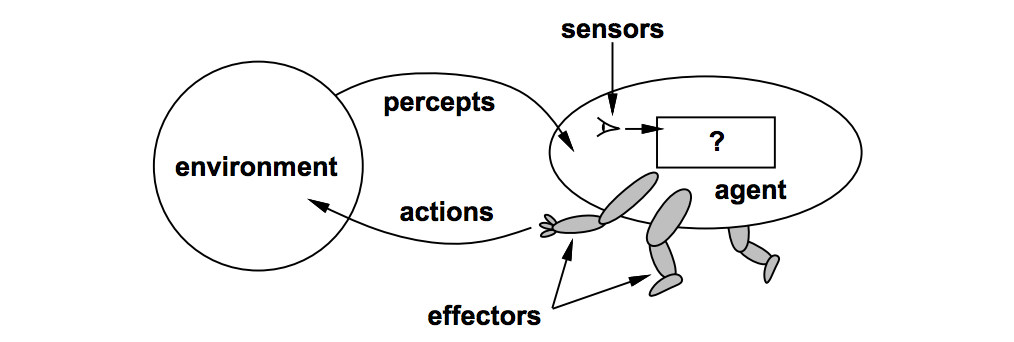
\includegraphics[scale=0.6]{intelligentagent.png}
	\caption{Illustration of an intelligent agent, taking from \cite[p.~32]{modernai1}}
	\label{fig:ia}
\end{figure}

An intelligent agent is an entity that uses \textbf{sensors} to perceive its \textbf{environment} and acts based on that perception through \textbf{actuators} or \textbf{effectors}. In software, this is often realised as an autonomous program or module that takes its perception of the  \textbf{environment} as input an returns \textbf{actions} as output. Figure \ref{fig:ia} shows the basic structure of an intelligent agent. \cite[p.~34]{modernai3}



\subsubsection{Rule-based systems}

A rule-based system decides \textbf{actions} from \textbf{inputs} as prescribed by a \textbf{ruleset} or \textbf{rule base}. A \textbf{semantic reasoner} is used to manage to the relationship between input and the ruleset. This follows a \textbf{match-resolve-act} cycle, which first finds all rules matching an input, chooses one based on a conflict strategy and then uses the rule to act on the input, usually in the form of an output. \cite[pp.~28-29]{rbsys}


\subsubsection{Reinforcement Learning}

A reinforcement learning agent focuses on a learning problem, with its goal to maximise \textbf{reward}. Given a current \textbf{state} the agent chooses an \textbf{action} available to it, which is determined by a \textbf{policy}. This action maps the current \textbf{state} to a new \textbf{state}. This \textbf{transition} is then evaluated for its \textbf{reward} . This \textbf{reward} often affects the \textbf{policy} of future iterations, but \textbf{policies} may be stochastic to some level. \cite[s.~1.3]{suttonrl}

\subsubsection{Online/Offline Learning}
\begin{description}
	\item[Offline] An offline (or batch) learner trains on an entire dataset before applying changes. 
	\item[Online] A online learner reacts/learns from data immediately after each datapoint.
\end{description} 
	
\subsubsection{Genetic Algorithms (GAs)}

Genetic Algorithms are an subset of evolutionary algorithms, a biologically inspired form of reinforcement learning. They model the solution as a \textbf{population} of \textbf{individuals}. Each \textbf{individual} has a set of \textbf{genes} (a  \textbf{genome}), which can be thought of as simple pieces of analogous information (most often in the form of bit strings). Each \textbf{individual} is assessed by some \textbf{fitness function}. This assessment can be used to cull the \textbf{population}, akin to survival of the fittest, or to increase the individual's chance of influencing the next \textbf{population}. The new \textbf{population} is created by \textbf{breeding}, using a combination of the following: \textbf{crossover} of the \textbf{genome} from two (or more) \textbf{individuals} (akin to sexual reproduction), \textbf{mutation} of the \textbf{genes} of one \textbf{individual} (akin to asexual reproduction) and \textbf{re-ordering} of the \textbf{genes} of one \textbf{individual}. Each new \textbf{population} is called a \textbf{generation}. \cite[p.~7]{mitchellga}

\subsubsection{Evolution Strategies (ESes)}

Evolution Strategies differ from standard Genetic Algorithms by using \textbf{truncation selection} before breeding. The top $\mu$ individuals of the population are chosen (usually by fitness) and bred to create $\lambda$ children. ES notation has the following form:  $\pmb{(\mu / \rho \  \overset{+}{,} \  \lambda)}$. $\rho$ denotes the number of individuals from $\mu$ used in the creation of a single $\lambda$, (i.e. number of parents of each child) this report will only consider the case $\rho = 1$. The $+$ and $,$ are explained below:  \cite[p.~6-10]{es-book} \cite[s.~4.1.2]{ecj-manual}
\begin{description}
	\item[$\pmb{(\mu \  , \   \lambda)}$]  Denotes an ES that has a population size of lambda. The top $\mu$ individuals are taken from the $\lambda$ in generation $g-1$, which then produce $\lambda$ children for generation $g$. This is done by creating $\lambda / \mu$ clones of each $\mu$ and then mutating them individually. 
	\item[$\pmb{(\mu  + \lambda)}$] Differs from the $\pmb{(\mu \  , \   \lambda)}$ variant by adding the $\mu$ individuals chosen from generation $g-1$ to the new generation $g$ after the mutation phase. Hence the population size is $\lambda + \mu$.
\end{description}

%-----------------------------------------------------------------------
% Reinforcement Learning in Games (Current Work in Field)
%-----------------------------------------------------------------------

\subsection{Reinforcement Learning Agents and Commercial Games}

\subsubsection*{Desirability}

Ventures in utilising reinforcement learning in commercial video games have been limited and largely ineffectual. However, there are many reasons why good execution of these techniques is desirable. Firstly, modern games have large and diverse player bases, having a game that can respond and personalise to a specific player can help cater to all. Secondly, learning algorithms produce agents that can respond well in new situations (over say FSMs or discrete logic), hence making new content easy to produce or generate. Lastly, humans must learn and react to environments and scenarios during games. Having non-playable characters do the same may produce a more believable, immersive and relatable AI, which is one of the key criticisms with current games. \cite[p.~7, p.~13]{panorama}

\subsubsection*{Issues}

The main issue with constructing effectual learning (or learnt) agent AI in game is risk versus reward. Game development works on strict cycles and there are limited resources to invest into AI research, especially if the outcome is uncertain. Furthermore, one player playing one game produces a very small data set, making learning from the player challenging. Moreover, AI that is believably human is a field still in its infancy. \cite{evolutioningamedesign}

\subsection{Reinforcement Learning Agents and Game AI Competitions}
\label{subsec:gameaicomps}

Despite the lack of commercial success, video games can act as great benchmark for reinforcement learning agents. They are designed to challenge humans, and therefore will challenge learning methods. Games naturally have some level of learning curve associated with playing them (as a human). Also, games require quick reactions to stimulus, something not true of traditional AI challenges such as board games. Most games have some notion of scoring suitable for a fitness function. Lastly, they are generally accessible to students, academics and the general public alike. \cite[p.~9]{panorama} \cite[p.~1]{marioaicomp} \cite[p.~2]{2012the}

Over the last few years several game based AI competitions have been run, over a variety of genres. These competitions challenge entrants to implement an agent that plays a game and is rated according to the competitions specification. They have attracted both academic \cite[p.~2]{2012the} and media interest \cite[p.~2]{marioaicomp}. The competition tend to encourage the use of learning techniques. Hence, several interesting papers concerning the application of reinforcement learning agents in video games have recently been published. Approaches tend to vary widely, modelling and tackling the problem very differently and specialising techniques in previously unseen ways. \cite[p.~11]{2012the}

Some brief details of the competitions which are of relevance to this project are compiled in to Table \ref{tab:gameaicomp}. The Mario AI Competition is also explored in more detail below.

\begin{table}
  \begin{adjustwidth}{-4cm}{-4cm}
  \begin{center} \small
    \begin{tabular}{ | >{\raggedright}p{2cm} | >{\raggedright}p{2cm} | p{7.5cm} |}
    \hline
    \textbf{Genre} & \textbf{Game} & \textbf{Description} \TBstrut \\ \thickhline
    Racing & TORCS (Open-source) \cite{torcs} &  
    \textbf{The Simulated Car Racing Competition}\newline Competitors enter agent drivers, that undergo races against other entrants which include qualifying and multi-car racing. The competition encourages the use of learning techniques. \cite{scrc}
      \\ \hline
    First Person Shooter (FPS) & Unreal Tournament 2004 &
    \textbf{The 2K BotPrize}\newline Competitors enter `bots' that play a multi-player game against a mix of other bots and humans. Entrants are judged on Turing test basis, where a panel of judges attempt to identify the human players. \cite{2kbot}
       \\ \hline
    Real Time Strategy (RTS) & Starcraft &
    \textbf{The Starcraft AI Competition}\newline Agents play against each other in a 1 on 1 knockout style tournament. Implementing an agent involves solving both micro objectives, such as path-planning, and macro objectives, such as base progression. \cite{starcomp}
       \\ \hline
    Platformer & Infinite Mario Bros (Open-source) &
    \textbf{The Mario AI Competition}\newline Competitors submit agents that attempt to play (as a human would) or create levels. The competition is split into `tracks', including Gameplay, Learning, Turing and Level Generation. In Gameplay, each agent must play unseen levels, earning a score, which is compared to other entrants. \cite{2012the} 
       \\ \hline
    
    \end{tabular}
  \end{center}
  \end{adjustwidth}
  \caption{This table summarises some recent game AI competitions \cite{2014how}}
  \label{tab:gameaicomp}
\end{table}

\subsubsection{The Mario AI Competition}

The Mario AI Competition, organised by Sergey Karakovskiy and Julian Togelius, ran between 2009-2012 and used an adapted version of the open-source game Infinite Mario Bros. From 2010 onwards the competition was split into four distinct `tracks'. We shall focus on the unseen Gameplay track, where agents play several unseen levels as Mario with the aim to finish the level (and score highly). \cite{marioaicomp} \cite{2012the}

\subsubsection*{\hspace{6pt}Infinite Mario Bros.}

Infinite Mario Bros (IMB) \cite{imb} is an open-source clone of Super Mario Bros.~3, created by Markus Persson. The core gameplay is described as a \emph{Platformer}. The game is viewed side-on with a 2D perspective. Players control Mario and travel left to right in an attempt to reach the end of the level (and maximise score). The screen shows a short section of the level, with Mario centred. Mario must navigating terrain and avoid enemies and pits. To do this Mario can move left and right, jump, duck and speed up. Mario also exists in 3 different states, \emph{small}, \emph{big} and \emph{fire} (the latter of which enables Mario to shoot fireballs), accessed by finding powerups. Touching an enemy (in most cases) reverts Mario to a previous state. Mario dies if he touches an enemy in the \emph{small} state or falls into a pit, at which point the level ends. Score is affected by how many coins Mario has collected, how many enemies he has killed (by jumping on them or by using fireballs or shells) and how quickly he has completed the level. \cite[p.~3]{2012the}

\subsubsection*{\hspace{6pt}Suitability to Reinforcement Learning}

The competitions adaptation of IMB (known henceforth as the `benchmark') incorporates a tuneable level generator and allows for the game to be sped-up by removing the reliance on the GUI and system clock. This makes it a great testbed for reinforcement learning. The ability to learn from large sets of diverse data makes learning a much more effective technique. \cite[p.~3]{2012the}

Besides that, the Mario benchmark presents an interesting challenge for reinforcement learning algorithms. Despite only a limited view of the ``world" at any one time the state and observable space is still of quite high-dimension. Though not to the same extent, so too is the action space. Any combination of five key presses per timestep gives a action space of $2^5$ \cite[p.~3]{2012the}. Hence part of the problem when implementing a learning algorithm for the Mario benchmark is reducing these search spaces. This has the topic of papers by Handa and Ross and Bagnell \cite{rossbagnell} separately addressed this issue in their papers \cite{handa} and \cite{rossbagnell} respectively.

Lastly, there is a considerable learning curve associated with Mario. The simplest levels could easily be solved by agents hard coded to jump when they reach an obstruction, whereas difficult levels require complex and varied behaviour. For example, traversing a series of pits may require a well placed series of jumps, or passing a group of enemies may require careful timing. Furthermore, considerations such as score, or the need to backtrack from a dead-end greatly increase the complexity of the problem. \cite[p.~3, p.~12]{2012the}


\subsection{Previous Learning Agent Approaches}
\label{ssec:prevagents}

Agent-based AI approaches in commercial games tend to focus on finite state machines, behaviour trees and rulesets, with no learning component. Learning agents are more prevalent in AI competitions and academia, where it is not only encouraged, but viewed as an interesting research topic \cite[p.~1]{marioaicomp}. Examples from both standpoints are compiled in Table \ref{tab:agents}.

\subsubsection{Evolutionary Algorithms}

Evolutionary algorithms are a common choice of reinforcement learning methods used in game-playing agents. D. Perez et al. note in their paper \cite[p.~1]{gramev} that they are particular suitable for game environments: 
\begin{quote}\itshape
`Their stochastic nature, along with tunable high- or low-level representations, contribute to the discovery of non-obvious solutions, while their population-based nature can contribute to adaptability, particularly in dynamic environments.'
\end{quote}
The evolutionary approach has been used across several genres of video games. For example, \emph{neuroevolution}, a technique that evolves neural networks, was used in both a racing game agent (by L. Cardamone \cite[p.~137]{scrc}) and a FPS agent (by the UT$\wedge$2 team \cite{2kbot}). Perhaps the most popular approach was to use genetic algorithms (GAs) to evolve a more traditional game AI agent. R. Small used a GA to evolve a ruleset for a FPS agent \cite{agentsmith}, T. Sandberg evolved parameters of a potential field in his Starcraft agent \cite{emapf} , \emph{City Conquest's} in-game AI used an agent-based GA-evolved build plan \cite{evolutioningamedesign} and D. Perez et al. used a grammatical evolution (a GA variant) to produce behaviour trees for a Mario AI Competition entry \cite{gramev}.

\subsubsection{Multi-tiered Approaches}

Several of the most successful learning agents take a multi-tiered approach. By splitting high-level behaviour from low-level actions agents can demonstrate more a complex, and even human-like, performance. For example, COBOSTAR, an entrant in the 2009 Simulated Car Racing Competition, used offline learning to determine high-level parameters such as desired speed and angle alongside a low-level crash avoidance module \cite[p.~136]{scrc}. UT$\wedge$2 used learning to give their FPS bot broad human behaviours and a separate constraint system to limit aiming ability \cite{2kbot}.  Overmind, the winner of the 2010 Starcraft Competition, planned resource use and technology progression at a macro level, but used A* search micro-controllers to coordinate units \cite{overmind}. 

\vspace{\baselineskip} \noindent
One learning agent that successfully utilised both an evolutionary algorithm and a multi-tiered approach is the Mario agent REALM, which is explored in more detail below. 

\subsubsection{REALM}
\label{ssec:realm}

The REALM agent, developed by Slawomir Bojarski and Clare Bates Congdon, was the winner of the 2010 Mario AI competition, in both the unseen and learning Gameplay tracks. REALM stands for \textbf{R}ule Based \textbf{E}volutionary Computation \textbf{A}gent that \textbf{L}earns to Play \textbf{M}ario. REALM went through two versions (V1 and V2), with the second being the agent submitted to the 2010 competition.

\subsubsection*{\hspace{6pt}Rule-based}

Each time step REALM creates a list of binary observations of the current scene, for example {\footnotesize IS\_ENEMY\_CLOSE\_LOWER\_RIGHT} and {\footnotesize IS\_PIT\_AHEAD}. Conditions on observations are mapped to actions in a simple ruleset. These conditions are ternary (either {\footnotesize TRUE}, {\footnotesize FALSE} or {\footnotesize DONT\_CARE}) \cite[p.~85]{realm}. A rule is chosen that best fits the current observations, with ties being settled by rule order, and an action is returned \cite[p.~86]{realm}.

Actions in V1 are explicit key-press combinations, whereas in V2 they are high-level plans. These plans are passed to a simulator, which reassesses the environment and uses A* to produce the key-press combination. This two-tier approach was designed in part to reduce the search space of the learning algorithm. \cite[pp.~85-87]{realm}

\subsubsection*{\hspace{6pt}Learning}

REALM evolves ruleset using an ES for 1000 generations. The best performing rule set from the final generation was chosen to act as the agent for the competition. Hence, REALM is an agent focused on offline learning. \cite[pp.~87-89]{realm}

Populations have a fixed size of 50 individuals, with each individual's genome being a ruleset. Each rule represents a gene and each individual has 20. Initially rules are randomised, with each condition having a 30\%, 30\%, 40\% chance to be {\footnotesize TRUE}, {\footnotesize FALSE} or {\footnotesize DONT\_CARE} respectively.

Individuals are evaluated by running through 12 different levels. The fitness of an individual is a modified score, averaged over the levels. Score focuses on distance, completion of level, Mario's state at the end and number of kills. Each level an individual plays increases in difficulty. Levels are predictably generated, with the seed being recalculated at the start of each generation. This is to avoid over-fitting and to encourage more general rules.

REALM used the $\pmb{(\mu  + \lambda)}$ variant ES, with $\mu = 5$ and $\lambda = 45$ (i.e. the best 5 individuals are chosen and produce 9 clones each). Offspring are exposed to: \textbf{Mutation}, where rule conditions and actions may change value; \textbf{Crossover}, where a rule from one child may be swapped with a rule from another child\footnote{This is similar to a  $\pmb{(\mu/\rho  + \lambda)}$ ES approach with $\rho = 2$, but crossover occurs in the mutation phase and between all children, rather than specifically with children from another parent.} and \textbf{Reordering}, where rules are randomly reordered. These occur with probabilities of 10\%, 10\% and 20\% respectively. \cite[pp.~88]{realm}

\subsubsection*{\hspace{6pt}Performance}

The REALM V1 agent saw a larger improvement over the evolution, but only achieved 65\% of the V2 agent's score on average. It is noted that V1 struggled with high concentrations of enemies and large pits. The creators also assert that the V2 agent was more interesting to watch, exhibiting more advanced and human-like behaviours. \cite[pp.~89-90]{realm}

The ruleset developed from REALM V2 was entered into the 2010 unseen Gameplay track. It not only scored the highest overall score, but also highest number of kills and was never disqualified (by getting stuck in a dead-end). Competition organisers note that REALM dealt with difficult levels better than other entrants. \cite[p.~10]{2012the}


\begin{table}
  \begin{adjustwidth}{-4cm}{-4cm}
  \begin{center} \small
    \begin{tabular}{ | >{\raggedright}p{2.2cm} | >{\raggedright}p{3.5cm} | p{6.8cm} |}
    \hline
    \textbf{Name} & \textbf{Game/Competition} & \textbf{Approach} \TBstrut \\ \thickhline
    
    M. Erickson \cite{2012the} & 2009 Mario AI Competition &
    A crossover heavy GA to evolve an expression tree.
    \\ \hline
    E. Speed \cite{2010the} & 2009 Mario AI Competition &
    GA to evolve grid-based rulesets. Ran out of memory during the competition.
    \\ \hline
    S. Polikarpov \cite[p.~7]{2010the} & 2009-10 The Mario AI Competition &
    Ontogenetic reinforcement learning to train a neural network with action sequences as neurons.
    \\ \hline
    REALM \cite{realm} & 2010 Mario AI Competition &
    GA to evolve rulesets mapping environment to high-level behaviour.
    \\ \hline
    D. Perez et al \cite{gramev} & 2010 Mario AI Competition &
    Grammatical evolution with a GA to develop behaviour trees. 
    \\ \hline
    FEETSIES \cite{feetsies} & 2010 Mario AI Competition &
    ``Cuckoo Search via L\'evy Flights" to develop a ruleset mapping an observation grid to actions. 
    \\ \hline
    COBOSTAR \cite[p.~136]{scrc} & 2009 Simulated Car Racing Competition &
    Covariance matrix adaptation evolution strategy to map sensory information to target angle and speed.
    Online reinforcement learning to avoid repeating mistakes.
    \\ \hline
    L. Cardamone \cite[p.~137]{scrc} & 2009 Simulated Car Racing Competition &
    Neuroevolution to develop basic driving behaviour.
    \\ \hline
    Agent Smith \cite{agentsmith} & Unreal Tournament 3 &
    GAs to evolve very simple rulesets, which determine basic bot behaviour.
     \\ \hline
    UT$\wedge$2 \cite{2kbot} & 2013 2K Botprize &
    Neuroevolution with a fitness function focused on being `human-like'.
    \\ \hline
    T. Sandberg \cite{emapf} & Starcraft &
    Evolutionary algorithms to tune potential field parameters.
     \\ \hline
    Berkeley Overmind \cite{overmind} & The Starcraft AI Competition &
    Reinforcement learning to tune parameters for potential fields and A* search.
    \\ \hline
    In-game Opponent AI \cite{evolutioningamedesign} & City Conquest &
    GAs to evolve build plans with fitness measured in a 1-on-1 AI match.
    \\ \hline
    In-game Creature AI\cite{blackandwhite} & Black \& White &
    Reinforcement Learning applied to a neural network representing the creatures desires.
    \\ \hline
    In-game Car AI \cite{projectgothamracing} & Project Gotham Racing &
    Reinforcement learning to optomise racing lines.
     \\ \hline
    
    \end{tabular}
  \end{center}
  \end{adjustwidth}
  \caption{Reinforcement learning agent-based approaches to game playing AI}
  \label{tab:agents}
\end{table}

\section{Project Specification}

\subsection{Aim}
The aim of the project is to explore the use of reinforcement learning techniques in creating a game-playing agent-based AI. This will be achieved by producing an intelligent agent, evolved by a genetic algorithm, that plays the Mario AI benchmark.

\subsection{Functional Requirements}
Functionally, the project can be split into three parts: the agent framework, which is responsible for gathering sensory information from the game and producing an action; level generation and playing, which is responsible for having an agent play generated levels with varying parameters; and the learning framework, which will apply a genetic algorithm to a representation of an agent, with an aim to improving its level playing ability. 

\subsubsection{Agent Framework}
The agent framework will conform to the interface supplied in the Mario AI benchmark\footnote{~Add agent interface code to appendix and link~}; receive the game \emph{Environment} and produce an \emph{Action}. It must be able to encode individual agents into a simple format (e.g. a bit string or collection of numbers). Additionally, it should be able to encode and decode agents to and from external files. 

The framework will be assessed in three ways. Firstly on its complexity, keeping the search space of the encoded agent small is important for the learning process. Secondly on its speed, the agent must be able to respond within one game tick. Thirdly on its capability, the framework must facilitate agents that can complete the easiest levels, and attempt the hardest ones. It is also required that human created agent encoding(s) be written (within the framework) to assist this assessment.

\subsubsection{Level Playing}
The level generation and playing package must be able to generate and play levels using an agent, producing a score on completion. It should extend the existing framework included in the Mario AI Benchmark software. Furthermore, it should be able to read parameters for generation and scoring from an external file.

The package will be evaluated on the level of variety in generated levels and the amount of information it can gather in order to score the agent.

\subsubsection{Learning Framework}
The learning framework should utilise a genetic algorithm to evolve an agent (in encoded form). It should also ensure that as many as possible of the parameters that govern the process can be held in external files, this included overall strategy as well fine grained detail (e.g. mutation probabilities and evaluation multipliers). Where impossible or inappropriate to hold such parameters externally it must be able to read them dynamically from their governing packages, for example boundaries on the agent encoding should be loaded from the agent package, rather than held statically in the learning framework. It must have the facility to report statistics from learning runs, as well as write out final evolved agents.

The learning framework will also be assessed on three counts. Firstly, learning should not run for too long, grating the freedom to increase generation count or adjust parameters. Secondly, the learning process should demonstrate a meaning improvement to the agent over generations as this demonstrates an effective genetic algorithm. Thirdly, the final evolved agent will be assessed, using the level playing package. It will tested against the human created agents and analysed for behaviours and strategies not considered during their creation. 

\subsection{Non-functional requirements}

Both the level playing package and the agent framework should not prevent or harm thread safety, allowing multi-threading in the learning framework. Each part should be deterministic, i.e. if given the same parameter files will always produce the same results. Lastly, The entire project must be able to be packaged and run externally.



\section{Design}

\section{Implementation}

\section{Testing}

\section{Evaluation}

\clearpage
\begin{thebibliography}{11}

\bibitem{myangelcafe}
  Siyuan Xu,
  \emph{History of AI design in video games and its development in RTS games},
  Department of Interactive Media \& Game development, Worcester Polytechnic Institute, USA,
  \url{https://sites.google.com/site/myangelcafe/articles/history_ai}.

\bibitem{pacmanghosts}
  Chad Birch,
  \emph{Understanding Pac-Man Ghost Behaviour},
  \url{http://gameinternals.com/post/2072558330/understanding-pac-man-ghost-behavior},
  2010.
  
\bibitem{halflife}
  Alex J. Champandard,
  \emph{The AI From Half-Like's SDK in Retrospective},
  \url{http://aigamedev.com/open/article/halflife-sdk/},
  2008.
  
\bibitem{fear}
  Tommy Thompson,
  \emph{Facing Your Fear},
  \url{http://t2thompson.com/2014/03/02/facing-your-fear/},
  2014.

\bibitem{halo}
  Damian Isla,
  \emph{GDC 2005 Proceeding: Handling Complexity in the Halo 2 AI},
  \url{http://www.gamasutra.com/view/feature/130663/gdc_2005_proceeding_handling_.php},
  2005.
  
\bibitem{rome}
  Alex J. Champandard,
 \emph{Monte-Carlo Tree Search in TOTAL WAR: Rome II Campaign AI},
 \url{http://aigamedev.com/open/coverage/mcts-rome-ii/},
 2014.
 
\bibitem{playermod}
  Georgios N. Yannakakis, Pieter Spronck, Daniele Loiacono and Elisabeth Andre,
  \emph{Player Modelling},
  \url{http://yannakakis.net/wp-content/uploads/2013/08/pm_submitted_final.pdf},
  2013.
  
\bibitem{skyrim}
  Matt Bertz,
  \emph{The Technology Behind The Elder Scrolls V: Skyrim},
  \url{http://www.gameinformer.com/games/the_elder_scrolls_v_skyrim/b/xbox360/archive/2011/01/17/the-technology-behind-elder-scrolls-v-skyrim.aspx},
  2011.
  
\bibitem{overmind}
  \emph{The Berkeley Overmind Project},
  University of Berkeley, California.
  \url{http://overmind.cs.berkeley.edu/}.
  
\bibitem{cellz}
  Simon M. Lucas,
  \emph{Cellz: A simple dynamical game for testing evolutionary algorithms},
  Department of Computer Science, University of Essex, Colchester, Essex, UK,
  \url{http://citeseerx.ist.psu.edu/viewdoc/download?doi=10.1.1.96.5068&rep=rep1&type=pdf}. 
  
\bibitem{panorama}
  G. N. Yannakakis and J. Togelius,
  \emph{A Panorama of Artificial and Computational Intelligence in Games},
  IEEE Transactions on Computational Intelligence and AI in Games,
  \url{http://yannakakis.net/wp-content/uploads/2014/07/panorama_submitted.pdf},
  2014.
  
\bibitem{marioaicomp}
  Julian Togelius, Noor Shaker, Sergey Karakovskiy and Georgios N. Yannakakis,
  \emph{The Mario AI Championship 2009-2012},
  AI Magazine 34 (3), pp. 89-92,
  \url{http://noorshaker.com/docs/theMarioAI.pdf},
  2013.

\bibitem{suttonrl}
  Richard S. Sutton and Andrew G. Barto,
  \emph{Reinforcement Learning: An Introduction}
  The MIT Press, Cambridge, Massachusetts, London, England,
  Available: \url{http://webdocs.cs.ualberta.ca/~sutton/book/ebook/the-book.html},
  1998.
  
\bibitem{modernai3}
  Stuart J. Russell, Peter Norvig,
  \emph{Artificial Intelligence: A Moden Approach (3rd ed.},
  Upper Saddle River, New Jersey,
  2009.
  
\bibitem{modernai1}
  Stuart J. Russell, Peter Norvig,
  \emph{Artificial Intelligence: A Moden Approach (1st ed.},
  Upper Saddle River, New Jersey,
  1995.
  
\bibitem{rbsys}
  Anoop Gupta, Charles Forgy, Allen Newell, and Robert Wedig,
  \emph{Parallel Algorithms and Architectures for Rule-Based Systems},
  Carnegie-Mellon University Pittsburgh, Pennsylvania,
  ISCA '86 Proceedings of the 13th annual international symposium on Computer architecture, pp.~28-37,
  1986.
  
\bibitem{mitchellga}
  Melanie Mitchell,
  \emph{An Introduction to Genetic Algorithms},
  Cambridge, MA: MIT Press,
  1996.

\bibitem{es-book}
  Hans-Georg Beyer and Hans-Paul Schwefel,
  \emph{Evolution Strategies: A Comprehensive Introduction},
  Natural Computing 1: 3?52,
  2002.

\bibitem{rlheli}
  Andrew Y. Ng, Adam Coates, Mark Diel, Varun Ganapathi, Jamie Schulte, Ben Tse, Eric Berger and Eric Liang,
  \emph{Inverted autonomous helicopter flight via reinforcement learning},
  International Symposium on Experimental Robotics,
  \url{http://www.robotics.stanford.edu/~ang/papers/iser04-invertedflight.pdf},
  2004.
  
\bibitem{rlhci}
  S. Singh, D. Litman, M. Kearns and M. Walker,
  \emph{Optimizing Dialogue Management with Reinforcement Learning: Experiments with the NJFun System},
  Journal of Artificial Intelligence Research (JAIR), Volume 16, pages 105-133, 2002,
  \url{http://web.eecs.umich.edu/~baveja/Papers/RLDSjair.pdf}.
  
\bibitem{evolutioningamedesign}
  Alex J. Champandard,
  \emph{Making Designers Obsolete? Evolution in Game Design},
  \url{http://aigamedev.com/open/interview/evolution-in-cityconquest/},
  2012.
  
\bibitem{blackandwhite}
  James Wexler,
  \emph{A look at the smarts behind Lionhead Studio's `Black and White' and where it can and will go in the future},
  University of Rochester, Rochester, NY 14627,
  \url{http://www.cs.rochester.edu/~brown/242/assts/termprojs/games.pdf},
  2002.
  
\bibitem{projectgothamracing}
  Thore Graepal (Ralf Herbrich, Mykel Kockenderfer, David Stern, Phil Trelford),
  \emph{Learning to Play: Machine Learning in Games},
  Applied Games Group, Microsoft Research Cambridge,
  \url{http://www.admin.cam.ac.uk/offices/research/documents/local/events/downloads/tm/06_ThoreGraepel.pdf}.
  
\bibitem{forza}
  \emph{Drivatar\texttrademark\ in Forza Motorsport},
  \url{http://research.microsoft.com/en-us/projects/drivatar/forza.aspx}.
  
\bibitem{2012the}
  Sergey Karakovskiy and Julian Togelius,
  \emph{Mario AI Benchmark and Competitions},
  \url{http://julian.togelius.com/Karakovskiy2012The.pdf},
  2012.
  
\bibitem{2010the}
  Julian Togelius, Sergey Karakovskiy and Robin Baumgarten,
  \emph{The 2009 Mario AI Competition},
  \url{http://julian.togelius.com/Togelius2010The.pdf},
  2010.
  
\bibitem{2014how}
  Julian Togelius,
  \emph{How to run a successful game-based AI competition},
  \url{http://julian.togelius.com/Togelius2014How.pdf},
  2014.
  
\bibitem{torcs}
  \emph{TORCS: The Open Racing Car Simulation},
  \url{http://torcs.sourceforge.net/}.

\bibitem{scrc}
  Daniele Loiacono, Pier Luca Lanzi, Julian Togelius, Enrique Onieva, David A. Pelta, Martin V. Butz, Thies D. L�nneker, Luigi Cardamone, Diego Perez, Yago S�ez, Mike Preuss, and Jan Quadflieg,
  \emph{The 2009 Simulated Car Racing Championship},
  IEEE Transactions on Computational Intelligence and AI in Games, VOL. 2, NO. 2,
  2010.
  
\bibitem{2kbot}
  \emph{The 2K BotPrize},
  \url{http://botprize.org/}
  
\bibitem{starcomp}
  Michael Buro, David Churchill,
  \emph{Real-Time Strategy Game Competitions},
  Association for the Advancement of Artificial Intelligence, AI Magazine, pp.~106-108,
  \url{https://skatgame.net/mburo/ps/aaai-competition-report-2012.pdf},
  2012.
  
\bibitem{imb}
  \emph{Infinite Mario Bros.},
  Created by Markus Perrson,
  \url{http://www.pcmariogames.com/infinite-mario.php}.
  
\bibitem{handa}
  H. Handa,
  \emph{Dimensionality reduction of scene and enemy information in mario},
  Proceedings of the IEEE Congress on Evolutionary Computation,  
  2011.
  
\bibitem{rossbagnell}
  S. Ross and J. A. Bagnell, 
  \emph{Efficient reductions for imitation learning},
  International Conference on Artificial Intelligence and Statistics (AISTATS),
  2010.
  
\bibitem{realm}
  Slawomir Bojarski and Clare Bates Congdon,
  \emph{REALM: A Rule-Based Evolutionary Computation Agent that Learns to Play Mario},
  2010 IEEE Conference on Computational Intelligence and Games (CIG '10) pp.~83-90.

\bibitem{gramev}
   D. Perez, M. Nicolau, M. O'Neill, and A. Brabazon,
   \emph{Evolving Behaviour Trees for the Mario AI Competition Using Grammatical Evolution},
   Proceedings of EvoApps, 2010, pp.~123-132.

\bibitem{feetsies}
  E. R. Speed, 
  \emph{Evolving a mario agent using cuckoo search and softmax heuristics},
  Proceedings of the IEEE Consumer Electronics Society's Games Innovations Conference (ICE-GIC), 2010,
  pp.~1-7.
  
\bibitem{emapf}
  Thomas Willer Sandberg,
  \emph{Evolutionary Multi-Agent Potential Field based AI approach for SSC scenarios in RTS games},
   University of Copenhagen,
   2011.
  
\bibitem{ecj}
  \emph{ECJ: A Java-based Evolutionary Computation Research System},
  \url{https://cs.gmu.edu/~eclab/projects/ecj/}.
  
\bibitem{ecj-manual}
  Sean Luke,
  \emph{The ECJ Owner's Manual, v23},
  \url{https://cs.gmu.edu/~eclab/projects/ecj/docs/manual/manual.pdf}
  George Mason University,
  2015.

\bibitem{astar}
  Robin Baumgarten,
  \emph{A* Mario Agent},
  \url{https://github.com/jumoel/mario-astar-robinbaumgarten}.
  
\bibitem{agentsmith}
  Ryan Small,
  \emph{Agent Smith: a Real-Time Game-Playing Agent for Interactive Dynamic Games},
  GECCO `08, July 12-16, 2008, Atlanta, Georgia, USA.
  \url{http://www.cs.bham.ac.uk/~wbl/biblio/gecco2008/docs/p1839.pdf}.

\end{thebibliography}
\end{document}

























